\chapter{The Standard Model and beyond}
\label{sec:Theory}
We know that we cannot describe all physical phenomena observed in nature within the framework of the Standard Model of Particle Physics (SM). There are several shortcomings of the model, which implies that we need an extension of the SM to understand and explain these problems. There are several different suggested theoretical solutions to these, and one of them is called supersymmetry (SUSY). SUSY introduces multiple new particles as an extension to the SM particles, but no SUSY particle has so far been detected. Many supersymmetric theories inlcude a weakly interacting massive particle (WIMPs) and thus a candidate to explain the dark matter (DM) in our Universe, a brief overview of which will be provided in this thesis. Before we discuss SUSY and DM, we begin with a run-through of the SM.
\section{The Standard Model}
\label{sec:SM}
The current best description we have of the fundamental constituents of our Universe is the Standard Model. It includes the elementary particles and the forces acting between them and can explain all visible matter we have around us (sans gravity). 

The particles in the SM are organized in three generations, as shown in figure \ref{fig:SM}. It consists of two different types of particles, namely fermions and bosons. Fermions are the matter particles, and the bosons carry the forces that act between the fermions and are usually called force particles. They are usually arranged in doublets according to their isospin, that describes their electroweak coupling. 

\begin{figure}[H]
    \centering
    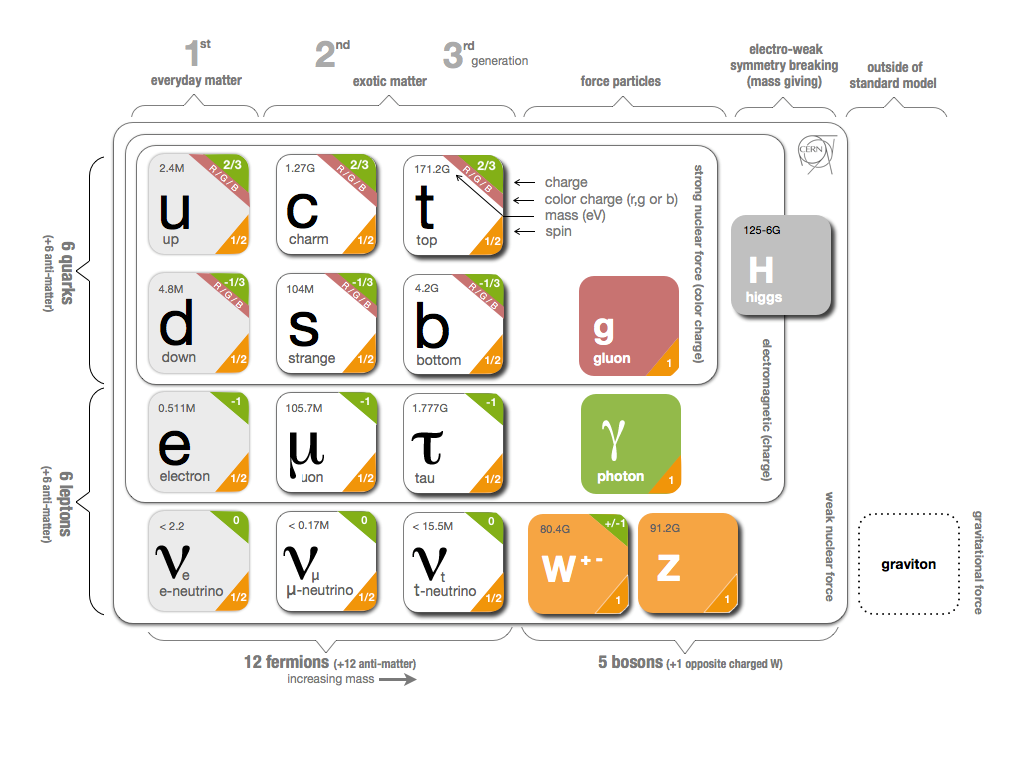
\includegraphics[width=\textwidth]{Figures/FromOnline/SM.png}
    \caption{An overview of the particles in the Standard Model \cite{SMpicture}.}
    \label{fig:SM}
\end{figure}

\subsection{Fermions}
If we look at figure \ref{fig:SM}, we can see that there are 12 different fermions split up in two groups called quarks and leptons, which again are split up into three generations. The lightest quarks and leptons are in the first generation, and the most massive quarks are in the third generation. All of the fermions are $\frac{1}{2}$-spin particles and differ by mass and electric charge. They also obey the Pauli exclusion principle, which means that only one fermion can occupy a given quantum state for any given set of quantum numbers.

\subsubsection{Quarks}
We have six different quarks \cite{thomson} in the SM, and they differ by mainly mass, but also charge (color charge, in addition to electrical charge). All the up-type quarks, which are the three quarks in the first row in figure \ref{fig:SM}, have charge +2/3 and all the down-type quarks, which is in the second row in figure \ref{fig:SM}, have charge -1/3. Since they carry a non-zero electric charge, they interact via the quantum electrodynamics (QED). They can also interact with the weak force which allows all possible combinations in doublets, where they differ by one unit of charge. 

\begin{align}
    \binom{u}{d} \text{,  } \binom{u}{s} \text{,  } \binom{u}{b} \text{,  } \binom{c}{d} \text{,  } \binom{c}{s} \text{,  } \binom{c}{b} \text{,  } \binom{t}{d} \text{,  } \binom{t}{s} \text{,  } \binom{t}{b}
\end{align}

The two quarks in the first generation, namely up (u) and down (d), are the constituents of the protons (uud) and neutrons (ddu) - which then combine in various ways to form atomic nuclei. The second and third generation of quarks (charm, strange, top and bottom) are more massive than the quarks in the first generation (up and down). Since the quarks in the second and third generations are more massive, they need more energy to exist and will therefore decay to lighter particles very fast. Quarks are the only known particles that interact with all the fundamental forces. They also carry color charge in addition to electrical and weak charge, which allows them to couple to different gluons through the strong interaction in quantum chromodynamics (QCD).  

Note that the quarks can be described by either mass eigenstates corresponding to the free-propagating Hamiltonian, or weak eigenstates corresponding to the way they interact under the weak interaction. Those sets of eigenstates do not coincide but are instead related to each other by the CKM matrix \cite{thomson}. 




\subsubsection{Leptons}
Leptons are the other six fermions in the SM. Like quarks, they come in three generations and are arranged in doublets, as shown below.

\begin{align}
    \binom{\nu_e}{e^-} \text{,  } \binom{\nu_\mu}{\mu} \text{,  } \binom{\nu_\tau}{\tau}
\end{align}

They also differ by mass and electric charge where the lower component has charge -1, and the upper has no charge. Because of that, neutrinos only interact with weak bosons, while for the electron, muon and, tau, electromagnetic interactions are also possible. In the SM the neutrinos are assumed to be massless, but we know from neutrino oscillation experiments that this is not true. However, exactly how the neutrinos acquire mass and why they are so much lighter than all of the other particles in the SM is not yet understood. 

Analogously to quarks, fermion mass and weak eigenstates do not coincide and they are related by the PMNS matrix \cite{thomson}. This phenomenon provides an explanation of neutrino oscillations, where after some distance from the interaction point we measure a different neutrino flavor. 


\subsection{Bosons}
On the right-hand side of figure \ref{fig:SM}, the integer spin particles (spin-1, spin-0) known as bosons \cite{thomson} are shown. Bosons follow Bose-Einstein statistics and contain the force carriers for the electromagnetic force, the weak force, and the strong force. If gravity was included in the Standard Model, it would have been through an extra boson, the graviton ($G$).

\subsubsection{The strong nuclear force}
The strong nuclear force is mediated by the gluon (g) \cite{thomson} and couples to the three color charges r, g, b. Moreover, as suggested by the name, it has a very strong coupling to quarks, and it is responsible for the fact that quarks do not appear as free, unbounded particles. The gluon is massless, and unlike the other forces, it can couple with itself, as you can see in the Feynman diagrams\footnote{Feynman diagrams are a way to graphically represent interactions between particles.} in figure\ref{fig:gluon_self_int}.

\begin{figure}[H]
    \centering
    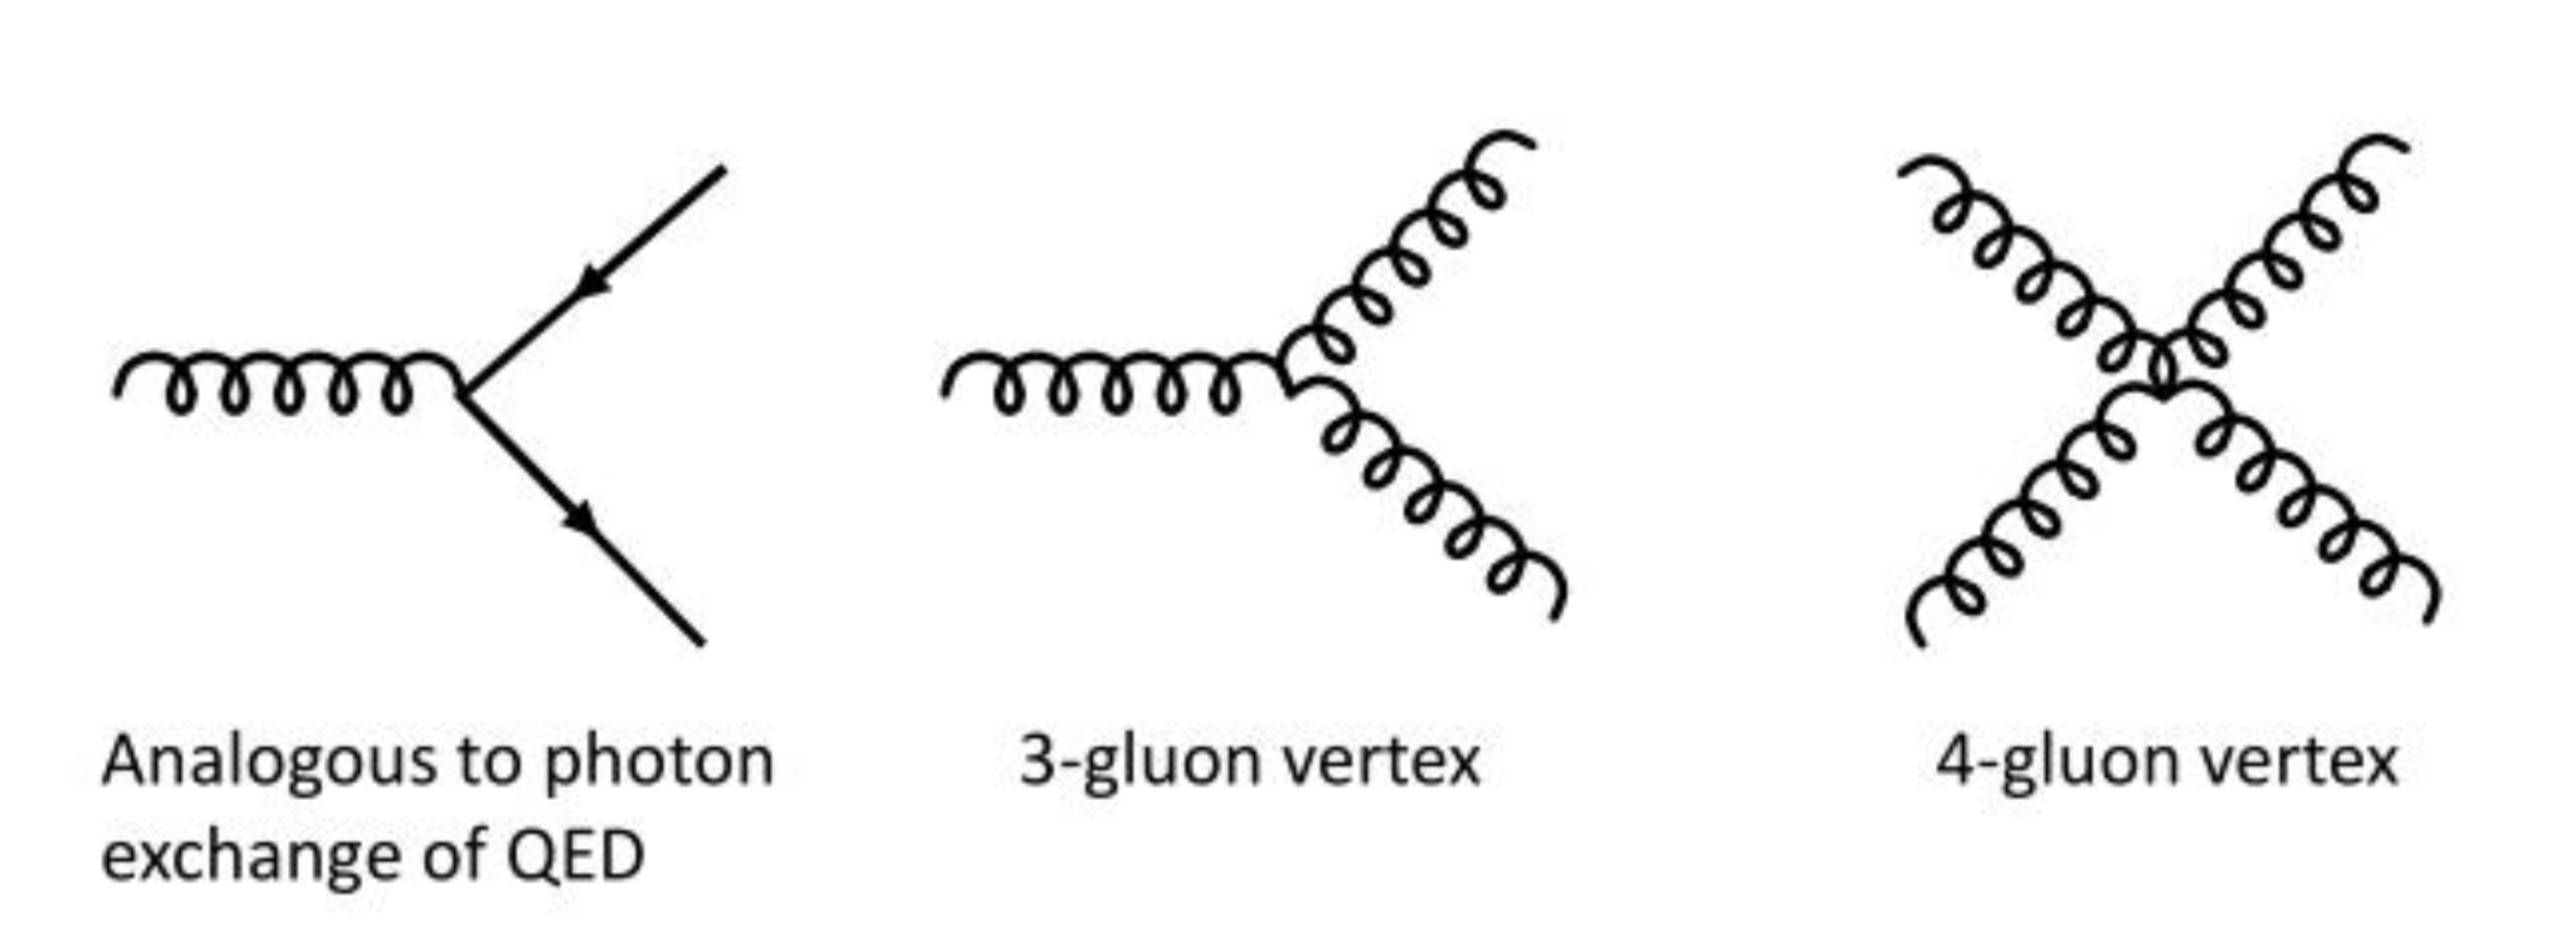
\includegraphics[width = \textwidth]{Figures/FeynmanDiagrams/gluon.pdf}
    \caption{Feynman diagrams for the strong force vertices, where the curly lines represent the gluons \cite{STRONGforce}.}
    \label{fig:gluon_self_int}
\end{figure}

\subsubsection{The electromagnetic force}
The electromagnetic force is mediated by the photon ($\gamma$) \cite{thomson} and couples to all fermions with electric charge, namely all the quarks and leptons except for the neutrinos. As for the gluon, it has no mass, but since it is electrical neutral it cannot couple to itself. 

\begin{figure}[H]
    \centering
    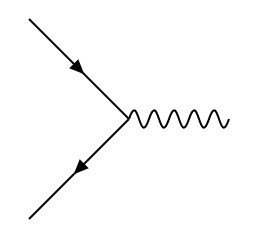
\includegraphics[width = 0.4\textwidth]{Figures/FeynmanDiagrams/photon.png}
    \caption{A Feynman diagram of the electromagnetic vertex, where the wiggly line represent the photon \cite{EMforce}.}
    \label{fig:my_label}
\end{figure}

\subsubsection{The weak nuclear forces}
The weak nuclear forces are mediated by the $W^\pm$-bosons and the $Z^0$-boson \cite{thomson}. They couple to all particles in the SM, and unlike the other force particles, they have mass. This feature is explained in the GWS model \cite{Xin2007GlashowWeinbergSalamMA} through a spontaneous symmetry breaking due to a non-zero vacuum expectation value that adds an extra degree of freedom to otherwise massless force carriers. It is also the only interaction known to allow flavor change, which means that e.g., an up quark can become a down quark or a muon become an electron as shown in figure\ref{fig:weak_force_FD}. 

\begin{figure}[H]
    \centering
    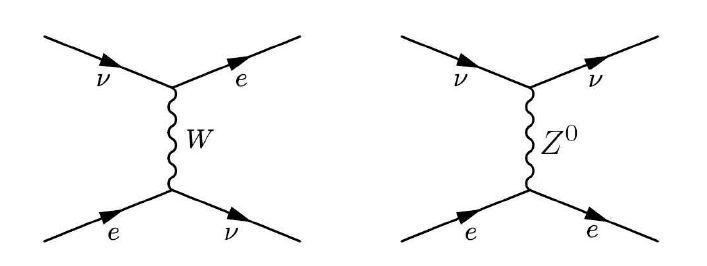
\includegraphics[width = 0.8\textwidth]{Figures/FeynmanDiagrams/weak.png}
    \caption{Feynman diagrams of the weak force vertices \cite{WEAKforce}.}
    \label{fig:weak_force_FD}
\end{figure}


\subsubsection{SM symmetries and the Higgs boson}
Formally, the three interactions in the nature are related by to three different symmetry groups. The SM is represented by

\begin{equation}
    U(1)_Y \otimes SU(2)_L \otimes SU(3)_C,
\end{equation}

where $U(1)_Y$ is the symmetry associated to the hyper charge $Y$, $SU(2)_L$ the transformations acting on the left-handed isospin doublets and $SU(3)_C$ are the ones acting on color triplets. The physical bosons $\gamma, Z^0, W^\pm$ are not the mediator associated to the single symmetry groups, but are instead a linear combination of those states explained by the spontaneous symmetry breaking leading to the electroweak theory. 

The final piece, the Higgs boson (H) \cite{thomson}, that was missing in the SM was discovered in 2012 at CERN \cite{Higgs_ATLAS, Higgs_CMS}. The discovery gives increased credence to the SM and explains why the weak force carriers, $Z^0$ and $ W^\pm $, have mass. The fermion masses, except for neutrinos, can also be explained by couplings to the Higgs boson. 




\section{Beyond the Standard Model}
As mentioned earlier, the SM is not enough to explain every phenomena observed in experiments. There are several challenging aspects of the SM; for instance, many of the parameters in the model are made to fit experimental data and do not come from theoretical principles. 
The SM does not offer a solution to unify the framework with gravity. The large difference between the weak energy scale and the Planck scale, known as the hierarchy problem, is another shortcoming of the SM. Moreover, the SM does not provide any explanation of the dark energy and dark matter observed in our Universe nor does it explain the small, but non-zero, masses of neutrinos.  

Given these shortcomings, various theories have been proposed addressing some of the open questions. Several extensions of the Standard Model exist, and there are pros and cons to all of them. Furthermore, even though the search has been going on for years, no concluding scientific evidence has been found to favor one particular SM extension over another. Below we detail an outline of one possibility: Supersymmetry.

\subsection{Supersymmetry}
\label{sec:SUSY}
One of the theories we are looking at is Supersymmetry (SUSY) \cite{sleptonexclusion}. SUSY relates the integer spin particles (bosons) and the half-integer spin particles (fermions) in the SM to half-integer spin particles and integer spin particles in SUSY. These new particles are named "super particles", or \textit{sparticles}, because SUSY predicts a supersymmetric partner for all of the SM particles. An illustration of the particles in SM and their superpartner in SUSY can be found in figure \ref{fig:smandsusy}.

\begin{figure}[H]
    \centering
    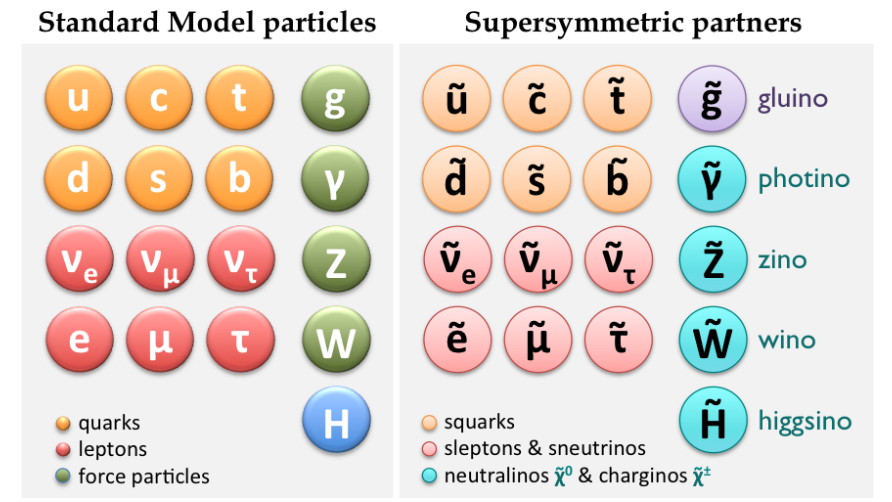
\includegraphics[width = 0.75\textwidth]{Figures/FromOnline/susy_particles.png}
    \caption{An illustration of the content of particles in the SM and sparticles in SUSY \cite{SUSYpic}.}
    \label{fig:smandsusy}
\end{figure}

In SUSY, we do not have to introduce any new gauge groups, which means we do not have to handle any new fundamental forces. Because of this we can, in a way, say that we can describe supersymmetry with the help of a supersymmetry operator $Q$ (shown in equation \ref{eq:SUSY}) that alters the spin of the SM particles by $1/2$ and commutes with the gauge transformations of the SM. 

\begin{equation}
    \label{eq:SUSY}
    Q\ket{fermions} = \ket{bosons} \text{,   }  Q\ket{bosons} =\ket{fermions}
\end{equation}

SUSY possibly provides a solution to the SM's hierarchy problem, which involves the need to reconcile the very different scales of electroweak symmetry breaking and the gravitational Planck scale ($M_{Pl}$). SUSY allows the unification of the electroweak and strong interactions, proposes dark matter particle candidates, and requires five Higgs bosons (three neutral and two charged ones). 




\begin{comment}

We know that the sparticles differ from the particles by $1/2$ spin, but that is almost the only difference when 

Supersymmetry allows for a connection between fermions and bosons by introducing a new set of particles. Each SM-particle has a sparticle, equal in all quantum numbers except a half unit difference in spin, i.e. the SM-fermions get a bosonic superpartner (denoted by an "s" in front of the name, e.g. electron $\rightarrow $ selectron) while the SM-bosons get a fermionic superpartner (denoted by "-ino" added to the end of the name, e.g. $W \rightarrow$ wino). All sparticles are denoted by a tilde above their symbol, e.g. selctron ($\tilde{e}$). If SUSY is a valid extension of the Standard Model, we know that it must be a broken symmetry where the particles and sparticles must have different masses although all the quantum numbers are equal. The sparticles must be heavier than their partner, or else we would already have been able to detect them in particle detectors, such as the ATLAS experiment. 

Supersymmetry offers a solution to the hierarchy problem, and when imposed as a local symmetry, gravity. According to Einsteins mass-energy equivalence equation ($E = mc^2$), we should be able to produce any particle in the universe as long as we collide them with a high enough amount of energy.





:
Production of pairs of sleptons, hypothetical supersymmetric partners of leptons, in the process pp→~l+~l-→ l+l-+χχ, where the DM candidate χ is the lightest neutralino (a mixture of photino, zino and higgsino), leading to a pair of leptons (e⁺e⁻ or µ⁺µ⁻) and missing transverse energy (MET).







The process I am looking at in this project is direct slepton production as shown in the Feynman diagram in figure \ref{fig:slepslep}. Production of pairs of sleptons, hypothetical supersymmetric partners of leptons, in the process $pp\rightarrow \tilde{l}^+\tilde{l}^- \rightarrow l^+l^-+ \chi \chi$, where the DM candidate $\chi$ is the lightest neutralino (a mixture of photino, zino and higgsino), leading to a pair of leptons ($e^+ e^-$ or $\mu^+ \mu^-$) and missing transverse energy (MET).



The same final state (l+l-+MET) above may be due to the production of a pair of lightest charginos χ±1 , a mixture of the wino (W-superpartner) and the charged higgsino (charged Higgs superpartner), through the process pp→ χ+1χ-1, followed by (i) slepton-mediated ( ~l+~l-/~ν~ν → l+l-  + ννbar + χχ) or (ii) W-mediated (W+W-→l+l-  + ννbar +χχ) decays into leptons and MET.



\textbf{To do:}
\begin{itemize}
    \item Fixing the hierarchy problem
    \item Superpartners
    \item Legg
\end{itemize}
\end{comment}





\subsection{Dark matter}
\label{sec:DM}
We have many unanswered mysteries in physics today, but probably the greatest one is the nature of dark matter (DM) \cite{monoZexclusion}. In the previous section's SUSY processes, we have seen that a "consequence" of SUSY may give us some viable DM candidates, namely the LSP neutralino. In this section, we will look at DM particles produced in a more simplified model; that is, a non-supersymmetry model. In this model, we assume that we have a DM mediator in addition to the DM particles in the final state. This mediator can be, among others, a scalar or a vector. This process's signature consists of detecting a well known SM particle recoiling against missing energy-momentum carried away by DM particles. 





\begin{comment}
\textbf{To do:}
\begin{itemize}
    \item Les om mørk materie. Du har jo strengt tatt ikke litt peiling engang..
    \item 
\end{itemize}


\begin{figure}[H]
    \centering
    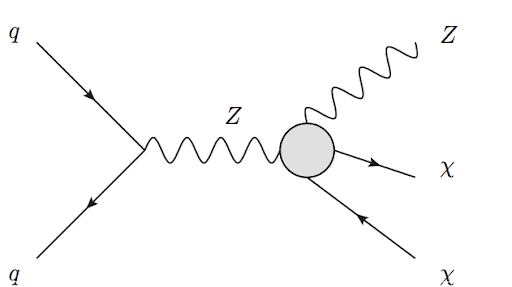
\includegraphics[width = 0.5\textwidth]{Figures/FeynmanDiagrams/monoZFeynman1.png}
    \caption{Caption}
    \label{fig:monoZFeynman1}
\end{figure}
\end{comment}






